\section{Présentation scientifique du travail}
\subsection{Introduction}
L'ARDrone 2.0 est un drone grand public Parrot dont nous allons présenter trois exploitations de failles de sécurité présentes au sein de celui-ci. Ces attaques seront présentées grâce à une application en Python appelée \textit{Krokmou}. La première attaque sera la prise de contrôle du drone par désauthentification du client, la seconde sera l'injection de commandes sur le drone et la dernière sera l'exploitation d'une connexion Telnet sur le drone.

\subsection{Premier pas avec le drone}
Dans un premier temps, après avoir allumé le drone, nous avons étudié celui-ci. La première chose que nous notons est que le drone crée un point d'accès Wifi (Access Point) afin que le client puisse se connecter à celui-ci et le contrôler au travers d'une application dédiée sur des supports Android, iOS ou PC. Toutefois, ce Wifi est un réseau ouvert et non sécurisé. Ainsi, toute personne disposant d'un matériel doté d'une carte Wifi et à portée Wifi du drone peut se connecter à celui-ci sans authentification. Toutes les communications entre le drone et le client sont donc en clair et non sécurisées. Cette faille facilite grandement l'accès au drone à l'attaquant qui n'a ainsi pas besoin de faire face à un réseau Wifi sécurisé pour accéder au drone. Ayant découvert cet accès facilité au drone, nous nous connectons à celui-ci avec un Linux et lançons un scan avec \textit{nmap} sur l'IP dur drone \begin{verbatim}192.168.1.1\end{verbatim} afin de connaître les ports ouverts sur le drone et découvrir des moyens d'accéder à celui-ci. Nous obtenons les resultats suivants:

\begin{figure}[H]
  \centering
  
\includegraphics[scale=0.3]{images/todo.png}
  \caption{Résultat du scan \textit{nmap} sur le drone}
\end{figure}

Nous observons un service \textbf{ftp} permettant de partager les vidéos filmées par le drone. Nous notons également un service \textbf{telnet} disponible sur le drone. Une rapide connexion à celui-ci, nous permet de voir que nous nous connectons sans identification au drone et, plus important, nous sommes \textbf{root} sur le drone ! Nous avons donc déjà potentiellement un contrôle total du drone car nous avons un accès illimité au système d'exploitation du drone.
\newline
Dans le même temps, nous nous documentons sur l'ARDrone 2.0. Grâce au SDK disponible sur le site \textbf{Parrot}, nous sommes en mesure de comprendre comment forger des commandes pour les envoyer au drone ainsi que les règles de contrôle du drone. Ainsi, nous savons que plusieurs clients peuvent être connectés au drone en même temps mais que c'est le premier qui envoie des paquets de commande UDP au drone qui en devient le "maître" et peut le contrôler.
\newline Après cette découverte du drone, nous établissons les trois scénarios d'attaques présentés en introduction que nous allons décrire par la suite.

\subsection{Prise de contrôle du drone par désauthentification du client}
La première attaque que nous allons présenter est une attaque permettant la prise de contrôle complète de l'ARDrone 2.0 en déconnectant le client légitime. Une fois connecté au réseau Wifi du drone, nous effectuons une désauthentification des clients connectés au drone grâce à \textbf{Aireplay} (cf Figure X.X).

\begin{figure}[H]
  \centering
  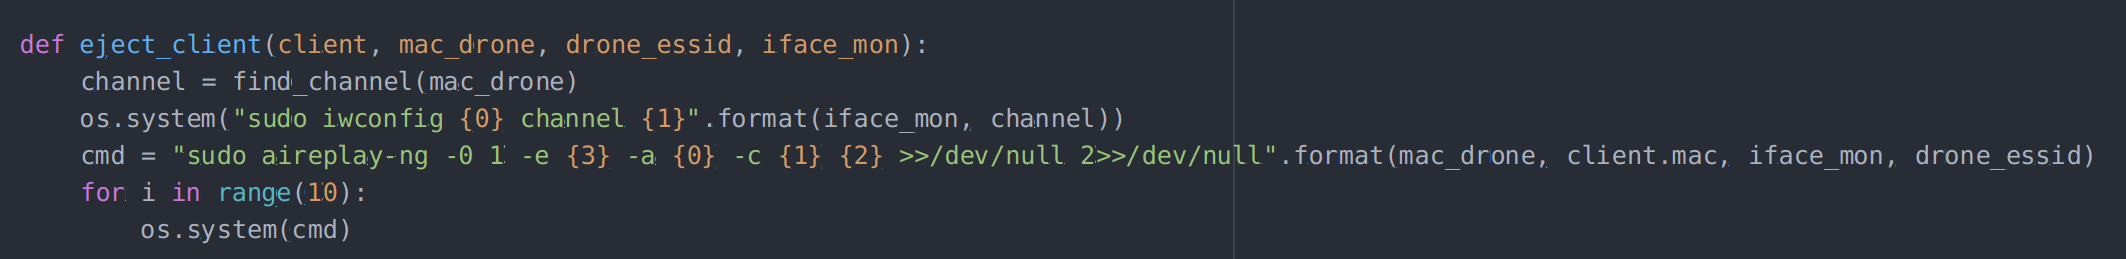
\includegraphics[scale=0.3]{images/aireplay.png}
  \caption{Utilisation d'\textbf{Aireplay} pour désauthentifier les clients}
\end{figure}

Une fois les clients désauthentifiés, nous nous reconnectons immédiatement au drone et sommes donc les premiers connectés au drone et les premiers à communiquer avec celui-ci donc "maître" du drone. Nous utilisons ensuite une application de contrôle via le navigateur web - disponible à l'adresse suivante: \url{https://github.com/functino/drone-browser} - afin de contrôler le drone avec le PC.

\subsection{Injection de commandes}
Cette seconde attaque a pour objectif d'injecter des commandes au drone sans en prendre le contrôle complètement. Le but est de faire exécuter certaines commandes tout en laissant le contrôle à l'utilisateur légitime.

\subsubsection{Liaison de commande}
La liaison de commande se fait entre le client et l'access point via le port \textbf{5556} en source et destination. Le client ne fait qu'envoyer régulièrement des paquets UDP pour maintenir et/ou commander le drone. Il n'y a pas de retour de la part du drone via cette liaison. Les informations à propos du drone sont envoyées par le drone vers le client via des paquets UDP sur le port \textbf{5554} en source et en destination. On va donc uniquement utiliser la liaison de commande pour injecter des commandes.

\subsubsection{Format des paquets UDP}
Pour créer des paquets de commandes légitimes, il faut étudier la forme de ceux-ci. Les paquets UDP transportent une chaîne de caractère qui sera interprétée par le drone.\\\\
Il faut que la chaîne de caractère commence par \textbf{AT*} puis vient le type de commandes :
\begin{itemize}
\item \textbf{REF} pour le décollage, atterrissage et le mode d'urgence
\item \textbf{PCMD} pour déplacer le drone
\item \textbf{PCMD\_MAG} pour déplacer le drone avec Absolute Control support
\item \textbf{FTRIM} régler la référence au plan horizontal (doit être au sol)
\item \textbf{CONFIG} configuration de l'AR Drone 2.0
\item \textbf{CONFIG\_IDS} identifiants pour les AT*CONFIG commandes
\item \textbf{COMWDG} réinitialise la communication
\item \textbf{CALIB} demande au drone de recalibrer le magnétomètre (doit être en vol) 
\end{itemize}
Dans notre cas, nous allons uniquement injecter des commandes \textbf{REF} et \textbf{PCMD}. Voyons le format des deux commandes.\\\\
Pour toutes les commandes, il faut que la chaîne de caractère soit suivi d'un \textbf{=} et d'un numéro de séquence. Le client incrémente ce numéro de séquence à chaque envoie de commande. Le drone valide uniquement les commandes donc le numéro de séquence est supérieur au précédent. Il faut donc prendre un numéro de séquence qui est au moins supérieur à celui en cours. Pour cela on prendra \textbf{10000000000} en numéro de séquence, ce qui nous assure de façon quasi-sûr d'être supérieur à celui en cours. On incrémentera également celui-ci à chaque envoie de commande injectée.\\\\
Pour \textbf{REF}, on va chercher à créer des ordres de décollage et d’atterrissage. Pour cela le numéro de séquence doit être suivi d'un argument qui sera égal à \textbf{290718208} pour le décollage et \textbf{290717696} pour l'atterrissage. Cela correspond à la modification du bit 9 de l'entier codé sur 32 bits.\\\\
On a donc \textbf{AT*REF=10000000000,290718208<CR>} pour le décollage et \textbf{AT*REF=}\\\textbf{10000000000,290717696<CR>} pour le décollage. On notera que les arguments doivent être séparés par une virgule et que la chaîne de caractère doit se terminer par un retour chariot noté <CR>.\\\\
Pour \textbf{PCMD}, il y a 5 arguments à la suite du numéro de séquence. Le premier informe si on utilise des commandes progressives et/ou le Combined Yaw mode, le second contrôle le déplacement gauche/droite, le troisième le déplacement avant/arrière, le quatrième le déplacement vertical et le cinquième la rotation selon l'axe vertical.\\\\
Pour le premier argument, on prend \textbf{1} ce qui correspond à l'activation du Combined Yaw mode.\\\\
Les autres arguments correspondent à une valeur entre -1 et 1. On demande donc au drone un pourcentage des limites de déplacement et de rotation défini dans la configuration du drone. On choisira une valeur de +/-0.3 pour avoir des commandes non trop sensibles. Cela correspond à passer l'argument +/-1050253722 qui est la représentation de 0.3 en nombre flottant à précision simple sur 32 bits puis en l'entier représenté sur 32 bits.\\\\
On a donc les commandes suivantes :
\begin{itemize}
\item Gauche \textbf{AT*PCMD=10000000000,1,-1050253722,0,0,0}
\item Droite \textbf{AT*PCMD=10000000000,1,1050253722,0,0,0}
\item Avancer \textbf{AT*PCMD=10000000000,1,0,-1050253722,0,0}
\item Reculer \textbf{AT*PCMD=10000000000,1,0,1050253722,0,0}
\item Descendre \textbf{AT*PCMD=10000000000,1,0,0,-1050253722,0}
\item Monter \textbf{AT*PCMD=10000000000,1,0,0,1050253722,0}
\item Tourner à gauche \textbf{AT*PCMD=10000000000,1,0,0,0,-1050253722}
\item Tourner à droite \textbf{AT*PCMD=10000000000,1,0,0,0,1050253722}
\end{itemize}

\subsubsection{Se faire passer pour le client légitime}
Pour connaître les différents clients connectés au drone, on scanne le réseau WiFi à l'aide de l'outil \textit{nmap}. On obtient alors le couple IP/MAC de chaque client. Pour être sûr de se faire passer pour le client légitime, on va envoyer notre paquet UDP en se fessant passer pour chaque client. Pour cela, on utilise \textit{scapy} qui permet d'envoyer nos paquets UDP avec l'adresse MAC et IP d'un des clients.

\subsubsection{Un contrôleur pour injecter des commandes}
Pour simplifier l'injection de commande, on a créé un contrôleur simpliste qui permet d'injecter les commandes vues précédemment.

\begin{figure}[H]
  \centering
  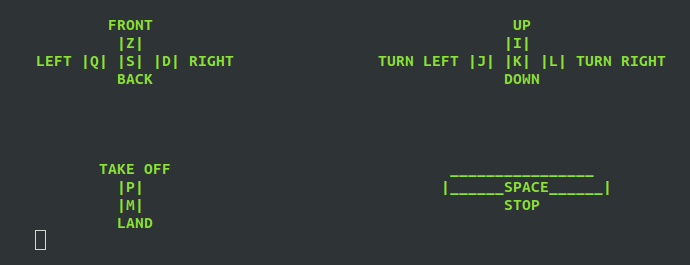
\includegraphics[scale=0.6]{images/injection_command_controler.png}
  \caption{Contrôleur pour l'injection de commande}
\end{figure}

Pour chaque commande, on envoie 3 paquets UDP avec un intervalle de 0.3 seconde. Cela est suffisant pour que le drone interprète notre commande.

\subsubsection{Conditions du maintient du contrôle par l'utilisateur légitime}
L'objectif de l'injection est de faire effectuer des commandes au drone tout en laissant le contrôle au client légitime. Or quand on envoie une commande avec un numéro de séquence 10000000000 ou plus, le numéro de séquence en cours du drone s'actualise à celui-ci. Le client légitime perd donc le contrôle du drone car son numéro de séquence est trop bas.\\
On va donc réinitialiser le numéro de séquence du drone à chaque fin d'injection de commande. Pour cela, il suffit d'envoyer une commande avec le numéro de séquence 1. On utilise alors la commande REF pour réinitialiser le numéro de séquence. On envoie 3 commandes REF à 0.3 seconde d'intervalle, décollage quand le drone est en vol et atterrissage quand le drone est au sol. Cela permet de ne pas avoir d'effet sur le drone autre que celui de réinitialiser le numéro de séquence.\\
Pour savoir l'état du drone, on considère que celui-ci est en vol au lancement de l'injection de commandes. En effet, les commandes de déplacement sont interprétées uniquement en vol. La seule commande valable au sol est la demande de décollage. On modifiera cet état en fonction des ordres d’atterrissage et de décollage des injections de commandes.\\
On notera que si le drone est dans un état autre que celui de l'utilisateur légitime alors ce dernier ne peut pas récupérer le contrôle du drone.


\subsection{Exploitation d'une connexion Telnet}
La dernière attaque exploite une vulnérabilité du drone. Un service \textbf{Telnet} est ouvert et permet d'accéder à un shell \textbf{root} sur le drone.

\begin{figure}[H]
  \centering
  
\includegraphics[scale=0.3]{images/todo.png}
  \caption{Accès \textbf{Telnet root} sur l'ARDrone 2.0}
\end{figure}

Ainsi une fois connecté au réseau du drone, n'importe qui peut utiliser cette connexion \textbf{Telnet} pour être administrateur sur le drone. Une fois le shell \textbf{root} obtenu, on se retrouve avec un accès au système d'exploitation du drone, qui est un \textbf{Linux}, et il est possible de faire ce que l'on veut. L'attaquant peut alors réaliser une large variété d'attaques directement sur le système d'exploitation. Il peut interagir avec les processus qui tournent sur celui-ci et notamment le processus qui pilote le drone \textbf{AJOUTER NOM PROCESSUS}.

\begin{figure}[H]
  \centering
  
\includegraphics[scale=0.3]{images/todo.png}
  \caption{Processus s'exécutant sur l'ARDrone 2.0}
\end{figure}

Il ainsi possible de modifier n'importe quel fichier du système d'exploitation et de réaliser par exemple un Déni de service sur le drone depuis "l'intérieur" de celui-ci. Etant \textbf{root} sur le drone sans nécessité d'escalade de privilèges, nous cherchons ce qui serait le plus intéressant de faire avec ce contrôle du drone. Nous décidons de démontrer la possibilité d'implanter un virus sur le drone. Ainsi nous avons développé un script en bash qui sera envoyé sur le drone par l'application \textit{Krokmou} accompagné d'un fichier au choix de l'attaquant. L'envoi se fait via la connexion \textbf{FTP} au drone. Une fois les deux fichiers sur le drone, l'application utilise la connexion \textbf{Telnet} afin d'exécuter le script. Celui-ci se copie alors au sein du dossier \begin{verbatim}/bin\end{verbatim} du drone et s'ajoute à la liste des processus à lancer au démarrage du drone afin qu'il s'exécute en permanence sur le drone. Le script va alors régulièrement essayer de copier le fichier envoyé par l'attaquant avec le script sur une clé USB qui serait connectée au drone. L'utilisateur légitime peut utiliser une clé USB pour récupérer des vidéos filmées par le drone et enregistrées sur celle-ci. Par défaut et à des fins de démonstration, le script dépose sur les clés USBs connectées une image.

\begin{figure}[H]
  \centering
  
\includegraphics[scale=0.3]{images/todo.png}
  \caption{Dépose du virus et du fichier par l'application}
\end{figure}

Cette attaque démontre que le drone peut facilement servir de vecteur d'attaque pour diffuser un virus par clé USB.
